\subsection{TCP Basics}
    \subsubsection*{Problems}
    \begin{enumerate}[label=\bfseries Problem \arabic*:,leftmargin=*,labelindent=1em]
    %addto counter에 앞서 subsection의 문제 개수만큼 적으면 자동으로 counting
    %image 번호만 신경써주면 된다.
    \addtocounter{enumi}{2}
    %%%%%%%%%%%%%%%%%%%%%%%%%%%%%%%%%%%%%%%%%%%%%%%%% Problem 1-3
        \item What is the sequence number of the TCP SYN segment that is used to initiate the TCP connection between the client computer and gaia.cs.umass.edu? What is it in the segment that identifies the segment as a SYN segment?\\[0.2mm]
        \soln The sequence number of TCP SYN segment that is used to initate the TCP connection of that is the no.1 Segement in filtered packet list by keyword, ‘TCP’ is the value of 0.\\
        We can figure out that segment is a SYN segment as that of TCP header contains Flags value.
    %     \vspace{-4mm}  
        \begin{figure}[!h]\centering
        \hspace{15mm}
    		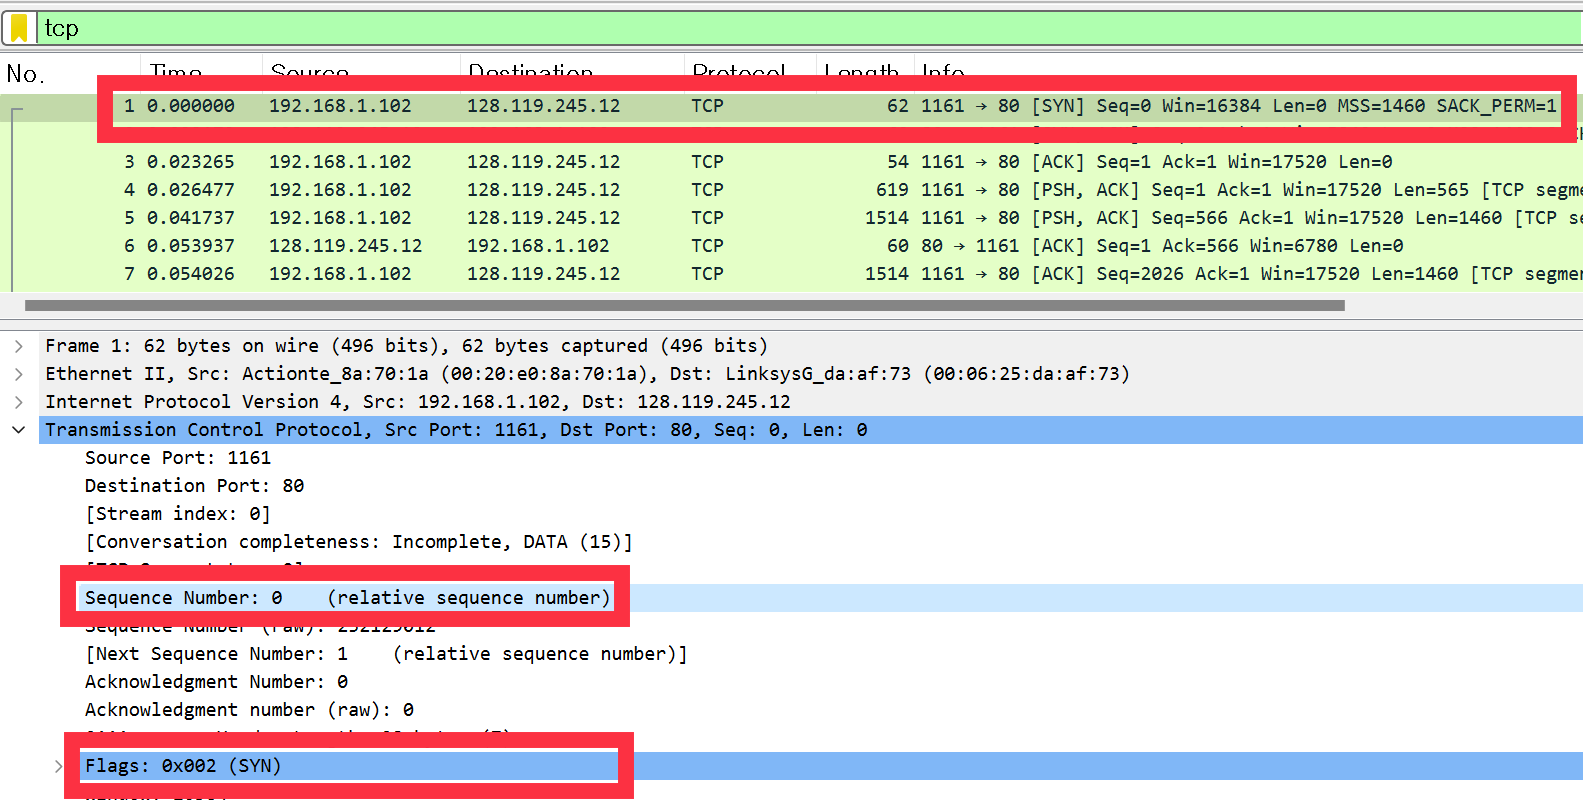
\includegraphics[width=.85\textwidth]{image/week02/1-3-1.png}
    		\caption{\footnotesize Problem 1-3's screenshot : Packet - [SYN] seq = 0’s TCP header}
    		\vspace{-10pt}
        \end{figure}
    %%%%%%%%%%%%%%%%%%%%%%%%%%%%%%%%%%%%%%%%%%%%%%%%% Problem 1-4
        \item What is the sequence number of the SYNACK segment sent by gaia.cs.umass.edu to the client computer in reply to the SYN? What is the value of the Acknowledgement field in the SYNACK segment? How did gaia.cs.umass.edu determine that value? What is it in the segment that identifies the segment as a SYNACK segment?\\[0.2mm]
        \soln The sequence number of the SYNACK segment is 0. \\\
        Acknowledgement field is the value of sequence number plus 1, 1.\\
        The message contains the information of this segment is the SYN,ACK segment as marked figure below.
    %     \vspace{-4mm}  
        \begin{figure}[!h]\centering
        \hspace{15mm}
    		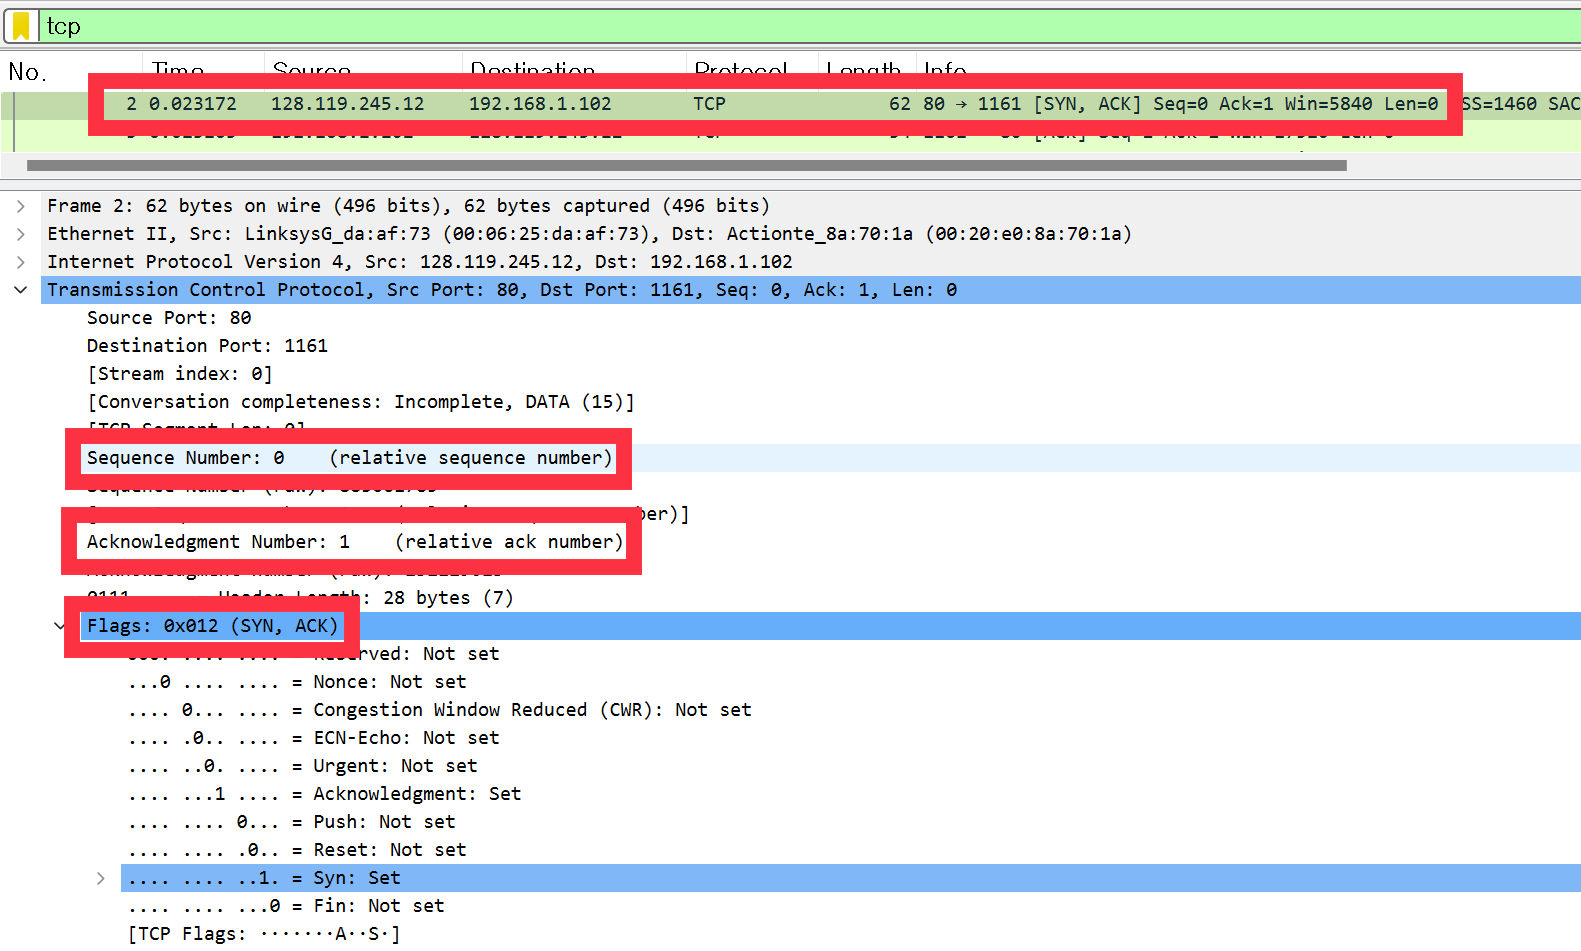
\includegraphics[width=.85\textwidth]{image/week02/1-4-1}
    		\caption{\footnotesize Problem 1-4's screenshot : Packet - HTTP POST’s TCP Header}
    		\vspace{-10pt}
        \end{figure}
    %%%%%%%%%%%%%%%%%%%%%%%%%%%%%%%%%%%%%%%%%%%%%%%%% Problem 1-5
        \item What is the sequence number of the TCP segment containing the HTTP POST command? Note that in order to find the POST command, you’ll need to dig into the packet content field at the bottom of the Wireshark window, looking for a segment with a “POST” within its DATA field.\\[0.2mm]
        \soln The sequence number of the TCP segment containing the HTTP POST command is 164041.
    %     \vspace{-4mm}  
        \begin{figure}[!h]\centering
        \hspace{15mm}
    		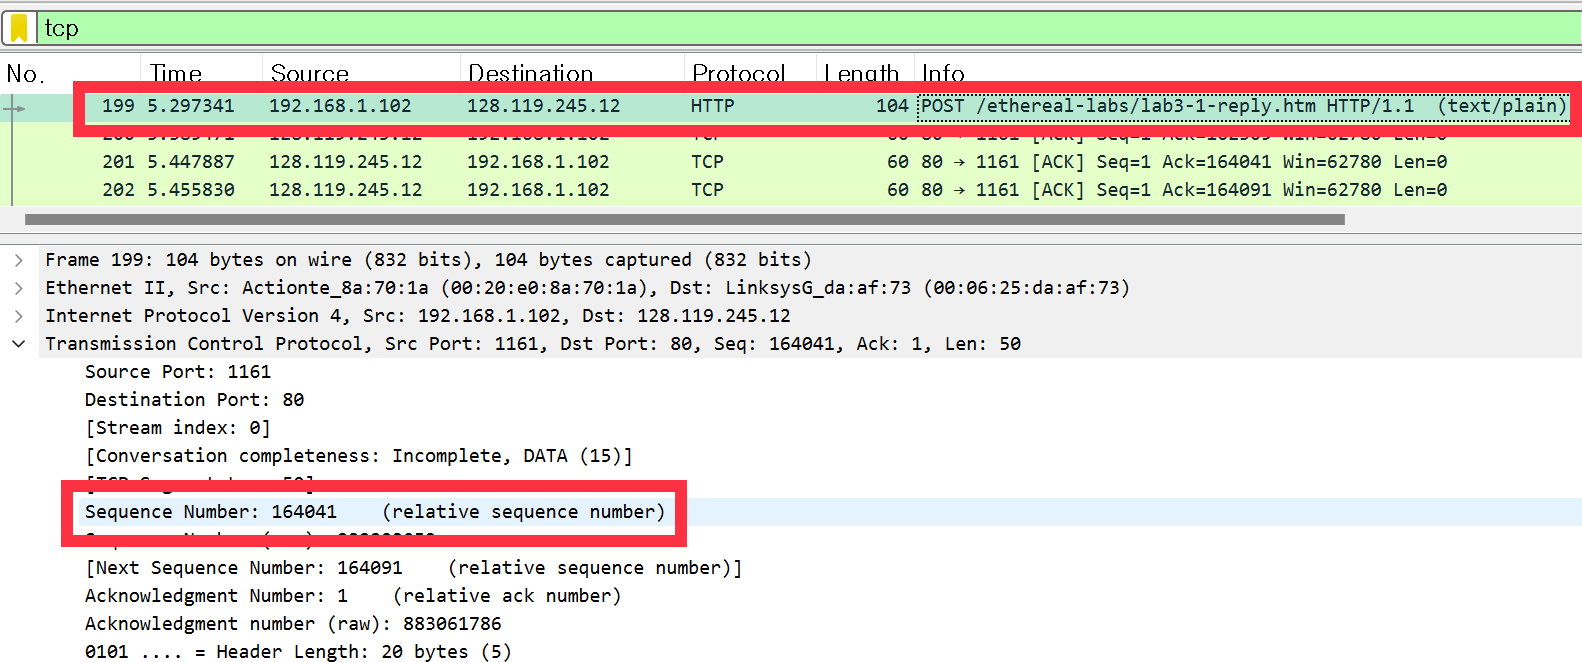
\includegraphics[width=.8\textwidth]{image/week02/1-5-1}
    		\caption{\footnotesize Problem 1-5's screenshot : Packet - HTTP POST’s TCP Header}
    		\vspace{-10pt}
        \end{figure}
    %%%%%%%%%%%%%%%%%%%%%%%%%%%%%%%%%%%%%%%%%%%%%%%%% Problem 1-6
        \item Consider the TCP segment containing the HTTP POST as the first segment in the TCP connection. What are the sequence numbers of the first six segments in the TCP connection (including the segment containing the HTTP POST)? At what time was each segment sent? When was the ACK for each segment received? Given the difference between when each TCP segment was sent, and when its acknowledgement was received, what is the RTT value for each of the six segments? \\
        What is the EstimatedRTT value after the receipt of each ACK?\\
        Assume that the value of the EstimatedRTT is equal to the measured RTT for the first segment, and then is computed using the EstimatedRTT equation below for all subsequent segments.\\
        \begin{equation*}
            \text{Estimated RTT} = 0.875 \times \text{Estimated RTT} + 0.125 \times \text{Sample RTT}
        \end{equation*}
        \soln
        The first six segements are No. 4,5,7,8,10,11. And those of sequence number are 1, 566, 2026, 3486, 4946, 6406.\\
        \vspace{-4mm}  
        \begin{figure}[!h]\centering
        \hspace{15mm}
    		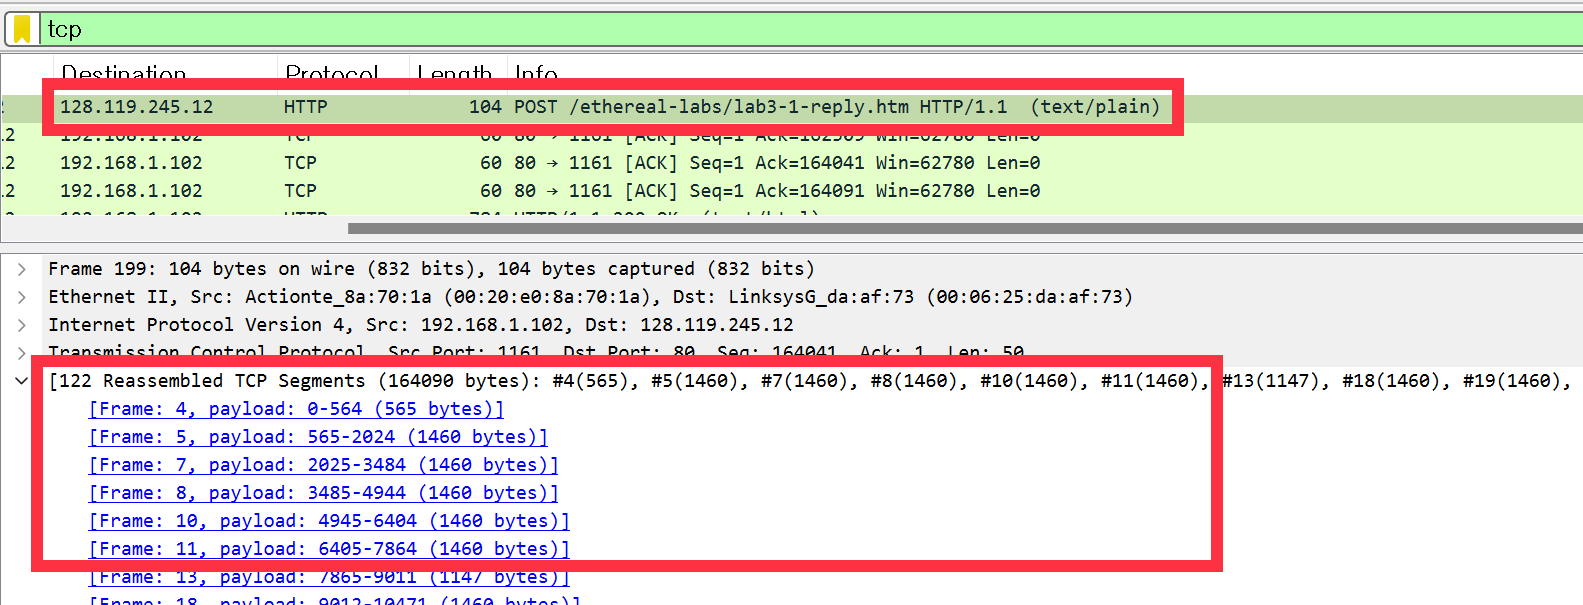
\includegraphics[width=.8\textwidth]{image/week02/1-6-1.png}
    		\caption{\footnotesize Problem 1-6-1's screenshot : }
    		\vspace{-10pt}
        \end{figure}    
        
        The time of segment sent, segment received the ACK, and the value of RTT are taken table below. To know each of six segment’s ACK received time, the No. of  ACKs that segemnts received are  No. 6, 9,12,14,15,16.
        \begin{table}[!h]\centering
        \hspace{10mm}
        \begin{tabular}{|l|c|c|c|}
        \hline
         & \multicolumn{1}{l|}{Sent Time} & \multicolumn{1}{l|}{Ack Received Time} & \multicolumn{1}{l|}{RTT (ACK Received TIme - Sent Time)} \\ \hline
        Segment 1 & 0.026477 & 0.053937 & 0.027460 \\ \hline
        Segment 2 & 0.041737 & 0.077294 & 0.035557 \\ \hline
        Segment 3 & 0.054026 & 0.124085 & 0.070059 \\ \hline
        Segment 4 & 0.054690 & 0.169118 & 0.114430 \\ \hline
        Segment 5 & 0.077405 & 0.217299 & 0.139890 \\ \hline
        Segment 6 & 0.078157 & 0.267802 & 0.189640 \\ \hline
        \end{tabular}
        \end{table}
\clearpage
        The estimated RTT is calculated by given equation.\\
        \vspace{-4mm}  
        \begin{figure}[!h]\raggedleft
        \hspace{15mm}
    		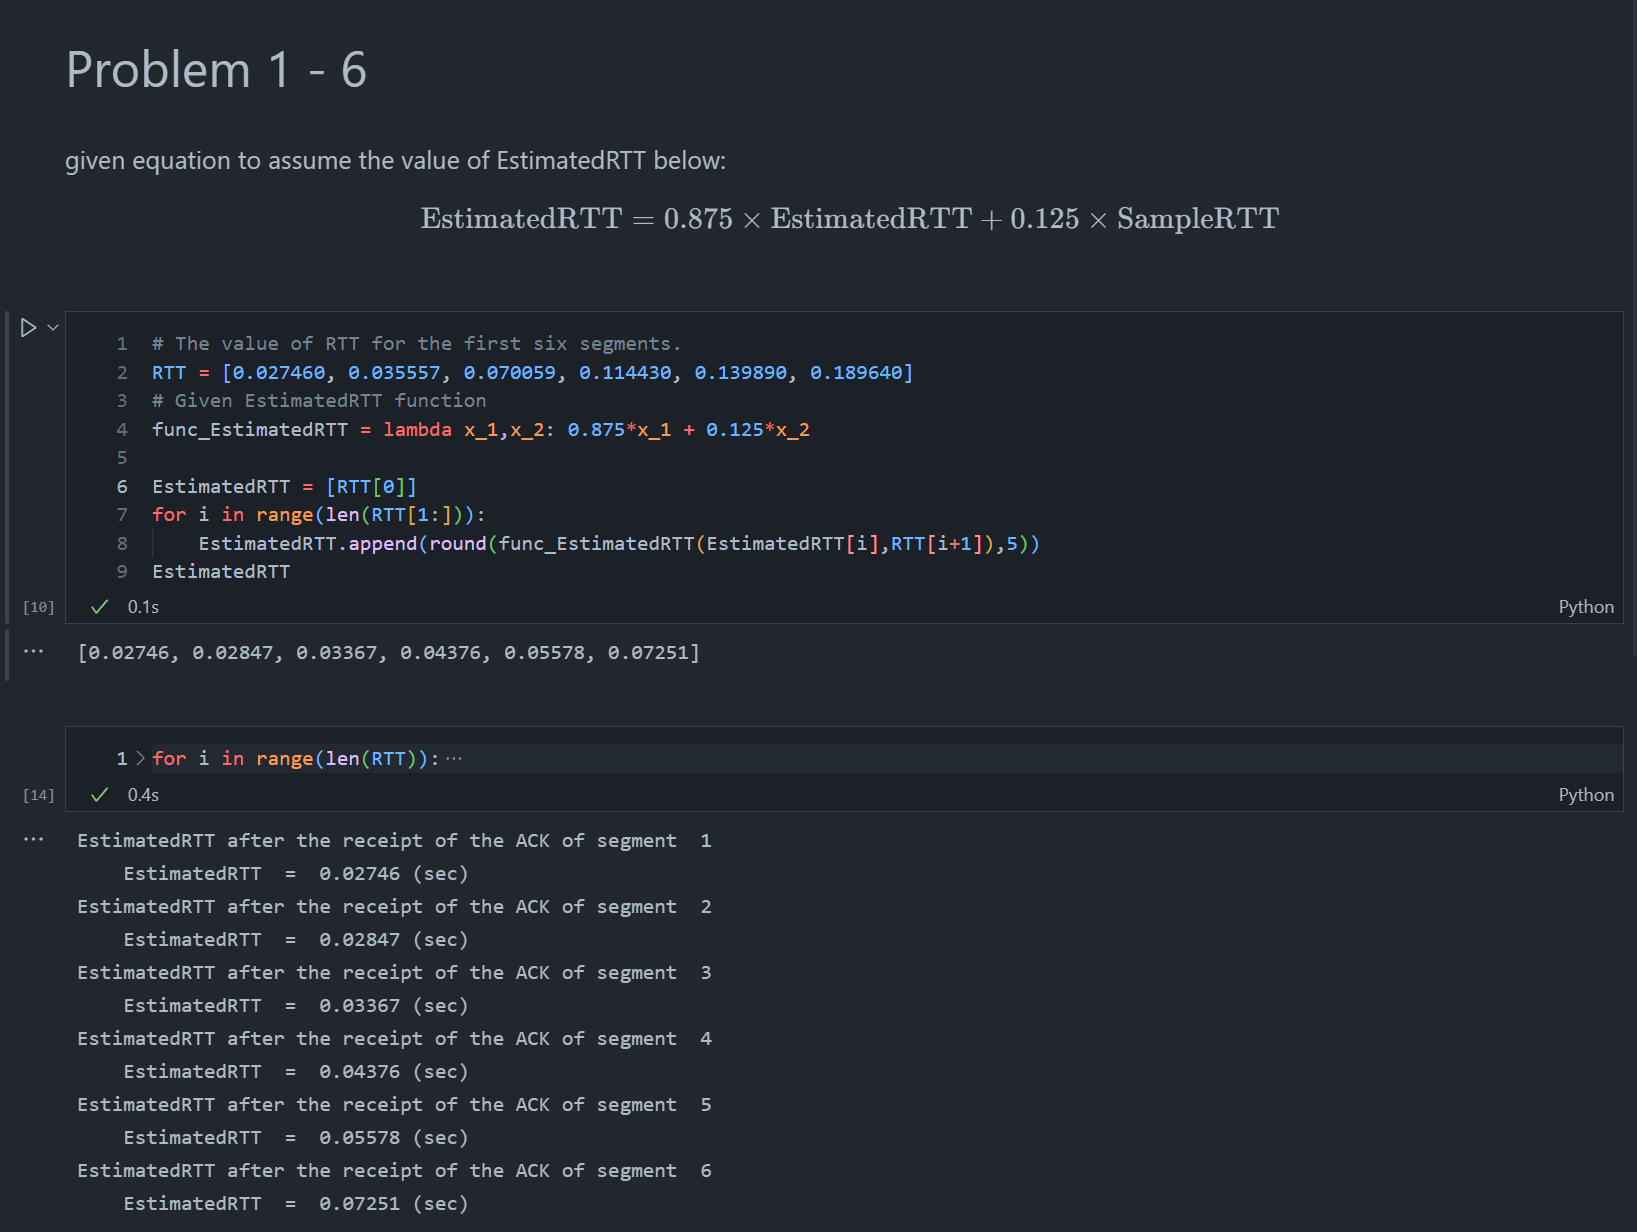
\includegraphics[width=.95\textwidth]{image/week02/1-6-3.png}
    		\caption{\footnotesize Problem 1-6-2's screenshot : The calculation result of EstimatedRTT by jupyter notebook}
    		\vspace{-10pt}
        \end{figure}
        
        We plot the RTT for each of the TCP segments that were being sent from the client to the gaia.cs.umass.edu.server.\\
        \vspace{-4mm}  
        \begin{figure}[!h]\raggedleft
        \hspace{15mm}
    		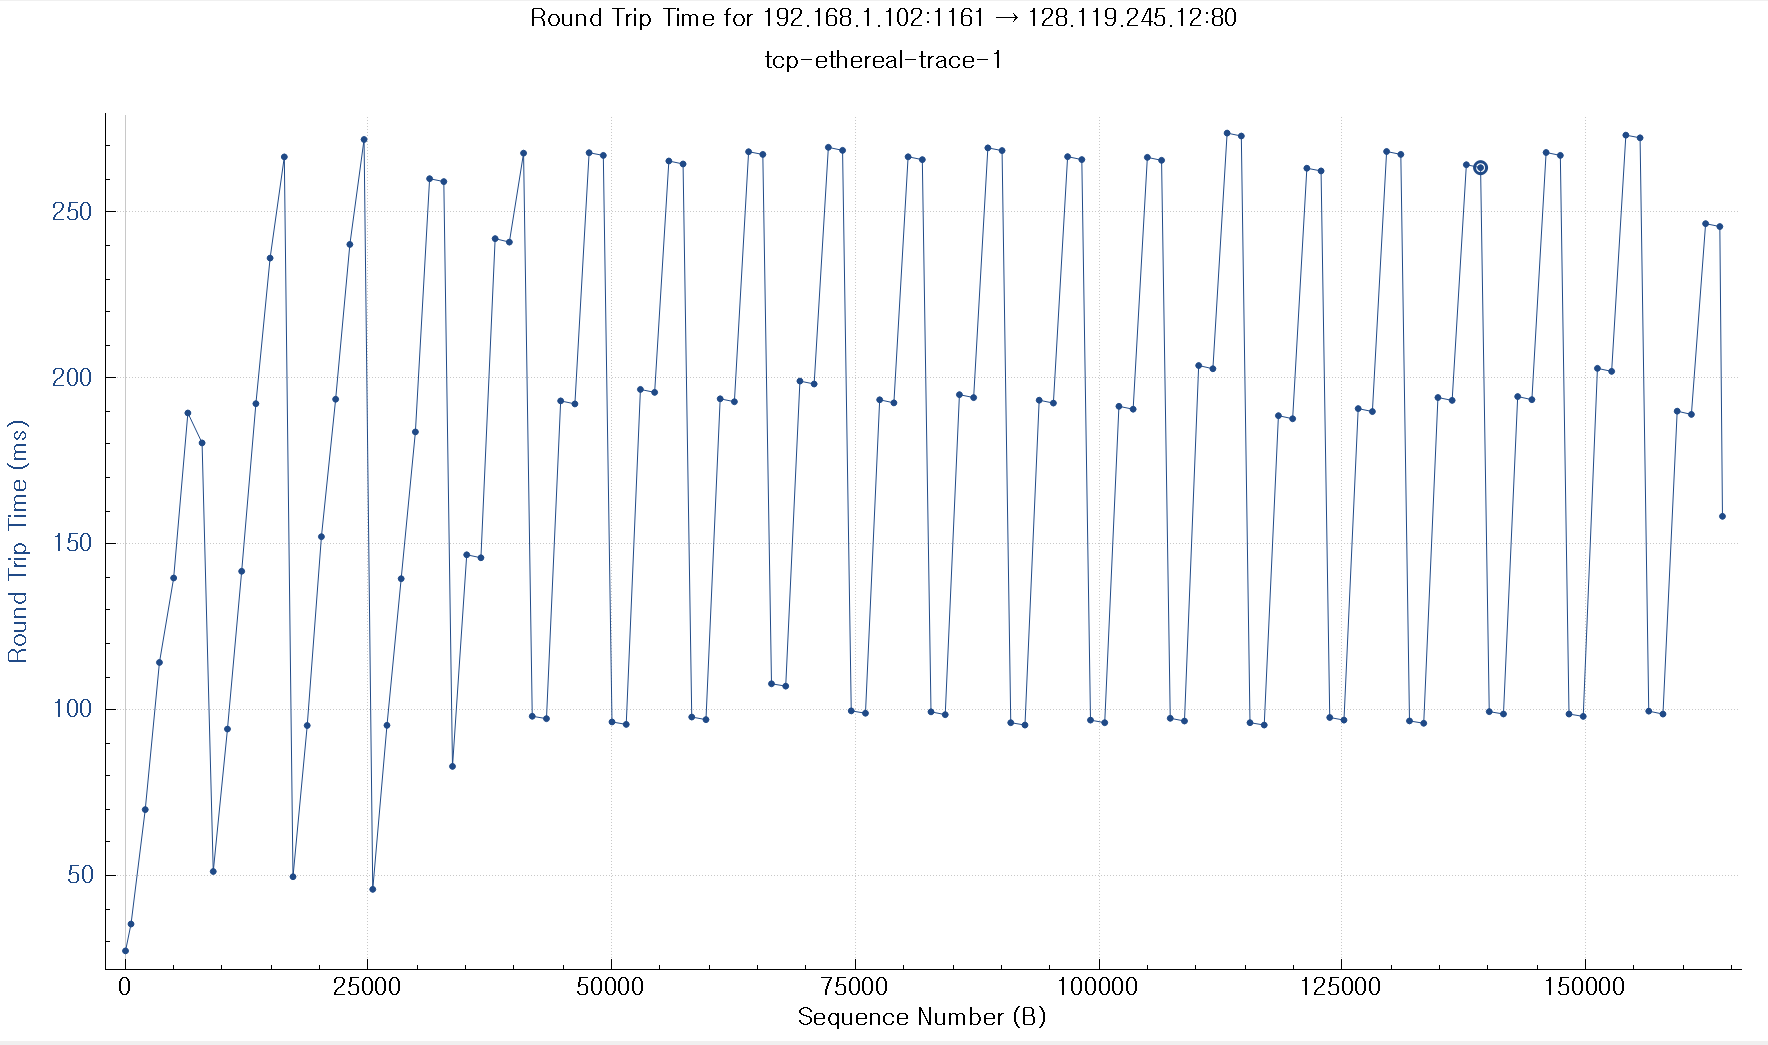
\includegraphics[width=.95\textwidth]{image/week02/1-6-2.png}
    		\caption{\footnotesize Problem 1-6-3's screenshot : RTT plot}
    		\vspace{-10pt}
        \end{figure}
\clearpage
    %%%%%%%%%%%%%%%%%%%%%%%%%%%%%%%%%%%%%%%%%%%%%%%%% Problem 1-7
        \item What is the length of each of the first six TCP segments?\\[0.2mm]
        \soln The length \footnote{’Len’ in packet info in Figure 9} of the fitst  TCP segments is 565, and the other TCP segments are 1460 as same.
    %     \vspace{-4mm}  
        \begin{figure}[!h]\centering
        \hspace{15mm}  
    		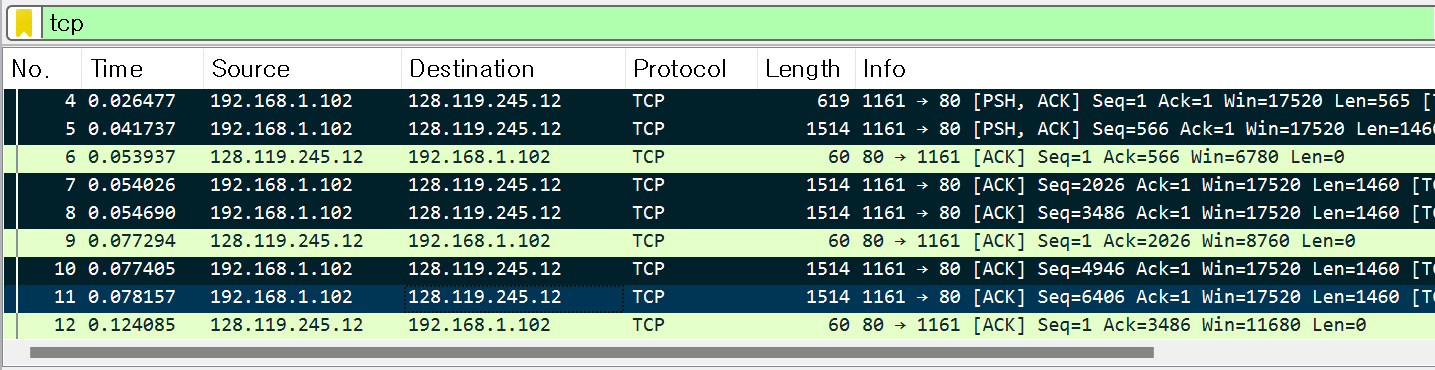
\includegraphics[width=.8\textwidth]{image/week02/1-7-1.png}
    		\caption{\footnotesize Problem 1-7's screenshot : Packet List - Marked the first six TCP segments, No.4, 5, 7, 8, 10, 11}
    		\vspace{-10pt}
        \end{figure}
    %%%%%%%%%%%%%%%%%%%%%%%%%%%%%%%%%%%%%%%%%%%%%%%%% Problem 1-8
        \item What is the minimum amount of available buffer space advertised at the received for the entire trace? Does the lack of receiver buffer space ever throttle the sender?\\[0.2mm]
        \soln The minimum amount of available buffer space advertised at the received for the entire trace be marked by the first ACK sent from the server. And the value is the window size value of the ACK. The first ACK, No.6 packet, of value is 6780.\\
        \vspace{-4mm}
        \begin{figure}[!h]\centering
        \hspace{15mm}  
    		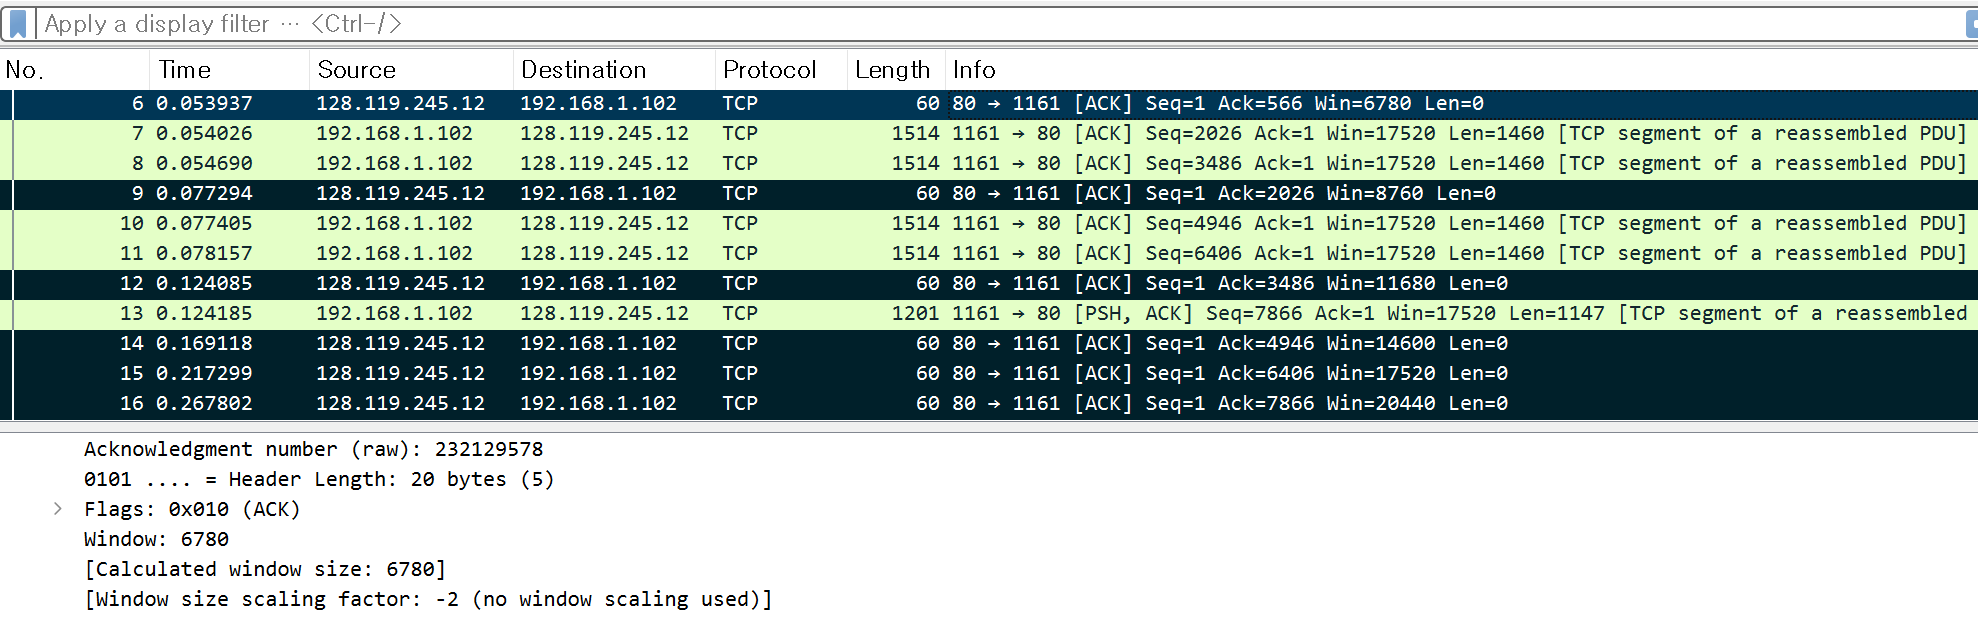
\includegraphics[width=.8\textwidth]{image/week02/1-8-1.png}
    		\caption{\footnotesize Problem 1-8's screenshot : Packet List - Marked the first six ACK, No.6, 9, 12, 14, 15, 16 with ACK No.6’s message}
    		\vspace{-10pt}
        \end{figure}
        
        Since we can find out that the first six ACK’s window size grows up to 20440 at ACK No.16 , and that means the maximum had not been reached in given trace. There was no throrrled because of the lack of receiver buffer space.
    %%%%%%%%%%%%%%%%%%%%%%%%%%%%%%%%%%%%%%%%%%%%%%%%% Problem 1-9
        \item Are there any retransmitted segments in the trace file? What did you check for (in the trace) in order to answer this question?\\[0.2mm]
        \soln
    %     \vspace{-4mm}  
        \begin{figure}[!h]\centering
        \hspace{15mm}  
    		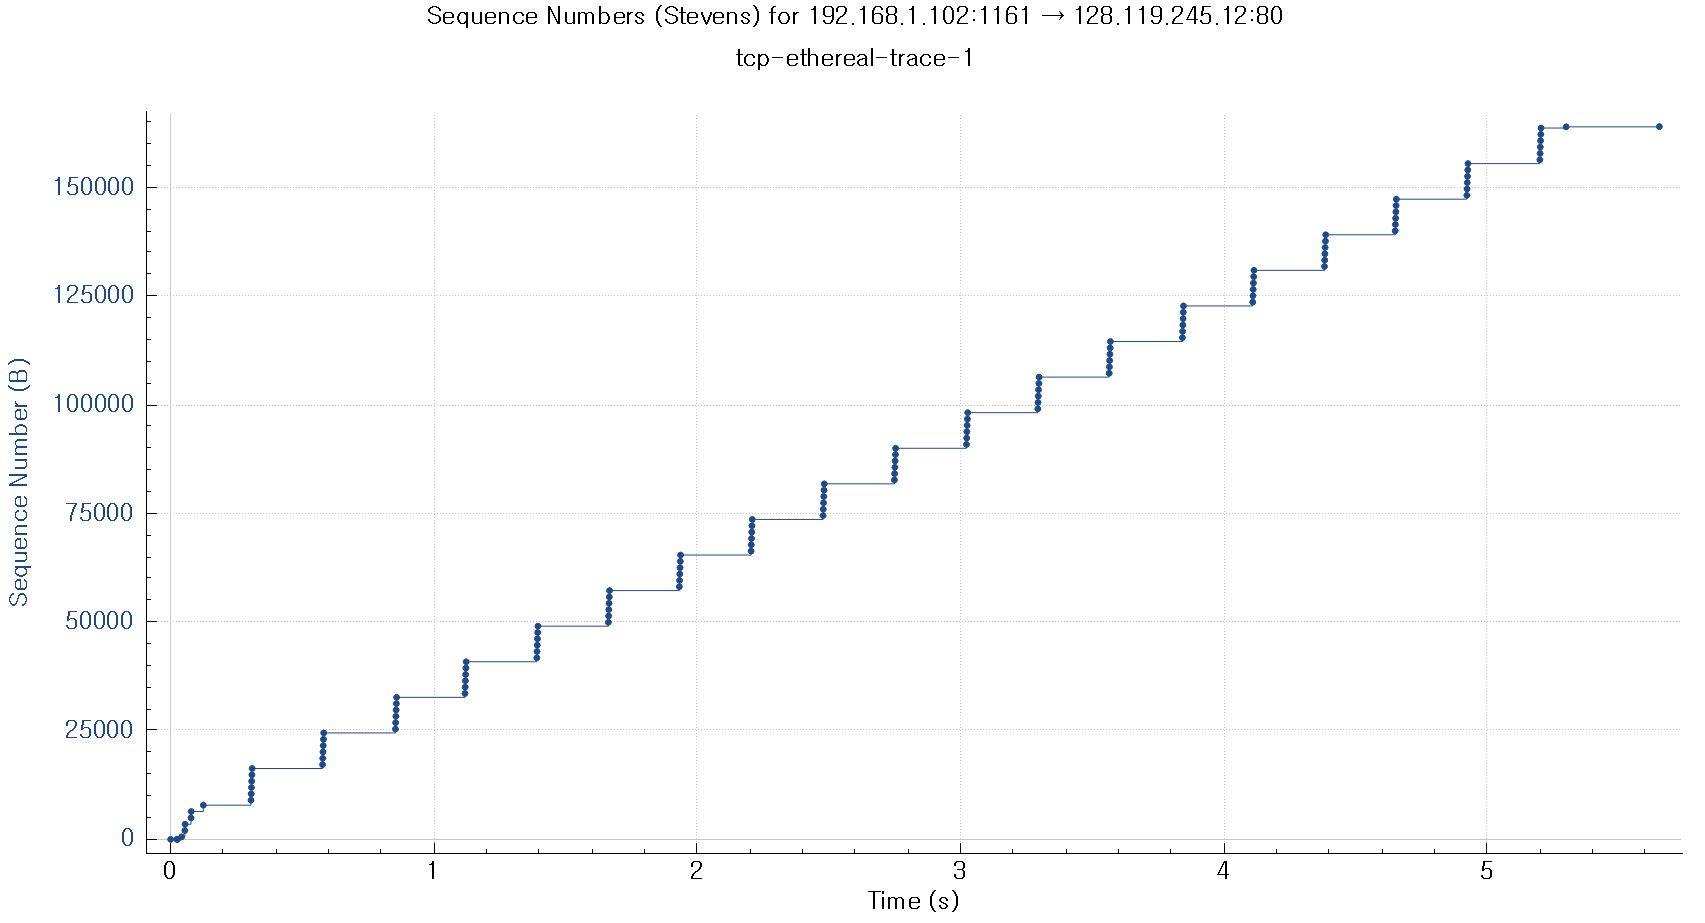
\includegraphics[width=.8\textwidth]{image/week02/1-9-1.png}
    		\caption{\footnotesize Problem 1-9's screenshot : }
    		\vspace{-10pt}
        \end{figure}
\clearpage
    %%%%%%%%%%%%%%%%%%%%%%%%%%%%%%%%%%%%%%%%%%%%%%%%% Problem 1-10
        \item How much data does the receiver typically acknowledge in an ACK? Can you identify cases where the receiver is ACKing every other received segment.\\[0.2mm]
        \soln
    %     \vspace{-4mm}  
    %     \begin{figure}[!h]\centering
    %     \hspace{15mm}  
    % 		\includegraphics[width=.85\textwidth]{image/week02/1-a-1.png}
    % 		\caption{\footnotesize Problem 1-10's screenshot : }
    % 		\vspace{-10pt}
    %     \end{figure}
% \newpage
    %%%%%%%%%%%%%%%%%%%%%%%%%%%%%%%%%%%%%%%%%%%%%%%%% Problem 1-11
        \item What is the throughput for the TCP connection? Explain how you calculated this value.\\[0.2mm]
        \soln
    %     \vspace{-4mm}  
    %     \begin{figure}[!h]\centering
    %     \hspace{15mm}  
    % 		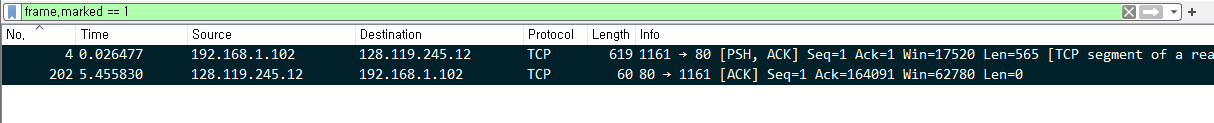
\includegraphics[width=.85\textwidth]{image/week02/1-b-1.png}
    % 		\caption{\footnotesize Problem 1-11's screenshot : }
    % 		\vspace{-10pt}
    %     \end{figure}
    \end{enumerate}
\newpage